\documentclass[10pt,a4paper]{report}
%\usepackage[latin1]{inputenc}
\usepackage[utf8]{inputenc}
\usepackage{amsmath}
\usepackage{amsfonts}
\usepackage{amssymb}
\usepackage{graphicx}
\usepackage{multicol}
\usepackage{tabularx}
\usepackage{tikz}
\usetikzlibrary{arrows,shapes,automata,petri,positioning,calc}
\usepackage{hyperref}
\usepackage{tikz}
\usetikzlibrary{matrix,calc}
\usepackage[margin=0.5in]{geometry}
\providecommand{\norm}[1]{\left\lVert#1\right\rVert}
\newcommand{\myvec}[1]{\ensuremath{\begin{pmatrix}#1\end{pmatrix}}}
\let\vec\mathbf

\newcommand{\mydet}[1]{\ensuremath{\begin{vmatrix}#1\end{vmatrix}}}

%\newcommand{\myvec}[1]{\ensuremath{\begin{pmatrix}#1\end{pmatrix}}}
%\let\vec\mathbf
\providecommand{\mtx}[1]{\mathbf{#1}}
\newenvironment{Figure}
  {\par\medskip\noindent\minipage{\linewidth}}
  {\endminipage\par\medskip}
\begin{document}
%--------------------logo figure-------------------------%
\begin{figure*}[!tbp]
  \centering
  \begin{minipage}[b]{0.4\textwidth}
   
\includegraphics[scale=0.05]{/sdcard/Download/FWC-main/iitlogo.jpg} 
  \end{minipage}
  \hfill
  \vspace{5mm}\begin{minipage}[b]{0.4\textwidth}
\raggedleft 
\includegraphics[scale=0.1]{/sdcard/Download/FWC-main/nrc.jpeg} 

  \end{minipage}\vspace{0.2cm}
\end{figure*}
%--------------------name & rollno-----------------------
\raggedright \textbf{Name}:\hspace{1mm}Prathyusha Korepu\hspace{3cm} \Large \textbf{Circle Assignment}\hspace{2.5cm} % 
\normalsize \textbf{Roll No.} :\hspace{1mm} FWC22047\vspace{1cm}
\begin{multicols}{2}


%----------------problem statement--------------%
\raggedright \textbf{Problem Statement:}\vspace{2mm}
\raggedright \\If a circle passes through the point (a,b) and cuts the circle $x^2+y^2=p^2$ orthogonally, then the equation of the locus of its centre is 

%(a)$x^2+y^2-3ax-4by+(a^2+b^2-p^2)=0$ \\
%(b)$2ax+2by-(a^2-b^2+p^2)=0$   \\
%(c)$x^2+y^2-2ax-3by+(a^2-b^2-p^2)=0$ \\
%(d)$2ax+2by-(a^2+b^2+p^2)=0$\\
\vspace{5mm}
 \vspace{2mm} 
\textbf{Construction} \\
\vspace{3mm}
{
\setlength\extrarowheight{2pt}
\begin{tabular}{|c|c|c|}
	\hline
	\textbf{Symbol}&\textbf{Value}&\textbf{Description}\\
	\hline
	$\vec{U_1}$ & $\begin{pmatrix}0 \\ 0 \\ \end{pmatrix}$ & center of given circle\\
	\hline
	$\vec{r_1}$ & 2 & radius of given circle\\ \hline
	$\begin{pmatrix}a & b \\ \end{pmatrix}$ & $\begin{pmatrix}1 & 2 \\ \end{pmatrix}$ & point on circle \\ \hline
\end{tabular}
} \\
 \vspace{2mm}
\textbf{Solution:}
\vspace{0.25cm}
With the given circle equation {$x^2+y^2=p^2$}, we can find out centre \(U_1\) and radius \(r_1\) of Circle-1 \\
\vspace{0.25cm}


Centre of Circle-1,

\begin{align} 
\vec{U_1} &= \begin{pmatrix}0 \\ 0 \\ \end{pmatrix} 
\end{align}


Radius of Circle-1,
\begin{align}
\vec{r_1=p}
\end{align}
The general form of conic is
\begin{align}
\vec{X}^{\top}\vec{V}\vec{X}+2\vec{U}^{\top}\vec{X}+\vec{f}=0
\end{align}
For circle 1  \\
\begin{align}
\vec{X}^{\top}\vec{V_1}\vec{X}+2\vec{U_1}^{\top}\vec{X}+\vec{f_1}=0
\end{align}
\begin{align}
\begin{pmatrix}x & y \\ \end{pmatrix} 
\begin{pmatrix}
1 & 0\\ 0 & 1 \\
\end{pmatrix}
\begin{pmatrix}x \\ y \\ \end{pmatrix}+2
\begin{pmatrix}0 & 0 \\ \end{pmatrix}
\begin{pmatrix}x \\ y \\ \end{pmatrix}+f1=0 \\
\end{align}
as circles are orthogonal 
\begin{align}
\vec{r_1}^2+\vec{r_2}^2=\vec{\norm{U_1-U_2}^2}
\end{align}
\begin{align}
\norm{U_1}^2+\norm{U_2}^2-2\vec{U_1}^{\top}\vec{U_2}=\vec{p}^2+\vec{r_2}^2
\end{align}
\begin{align}
\vec{r_2}^2=\vec{\norm{U_2}}^2-\vec{f_2}
\end{align}
By solving the equations (6) and (7)
\begin{align}
\vec{f_2}=\vec{p}^2
\end{align}
For circle 2 \\
\begin{align}
\vec{X}^{\top}\vec{V_2}\vec{X}+2\vec{U_2}^{\top}\vec{X}+\vec{f_2}=0
\end{align}

\begin{align}
\begin{pmatrix}x & y \\ \end{pmatrix} 
\begin{pmatrix}
1 & 0\\ 0 & 1 \\
\end{pmatrix}
\begin{pmatrix}x \\ y \\ \end{pmatrix}+2
\begin{pmatrix}-g & -t \\ \end{pmatrix}
\begin{pmatrix}x \\ y \\ \end{pmatrix}+p^2=0 
\end{align}
\begin{align}
\vec{x}^2+\vec{y}^2-\vec{2gx}-\vec{2ty}+\vec{p}^2=0
\end{align}
By substituting (a,b) in equation (13) \\
\begin{align}
\vec{a}^2+\vec{b}^2-\vec{2ga}-\vec{2tb}+\vec{p}^2=0
\end{align} 
The locus is \\
\begin{align}
\vec{2ga}+\vec{2tb}-(\vec{a}^2+\vec{b}^2+\vec{p}^2)=0
\end{align}
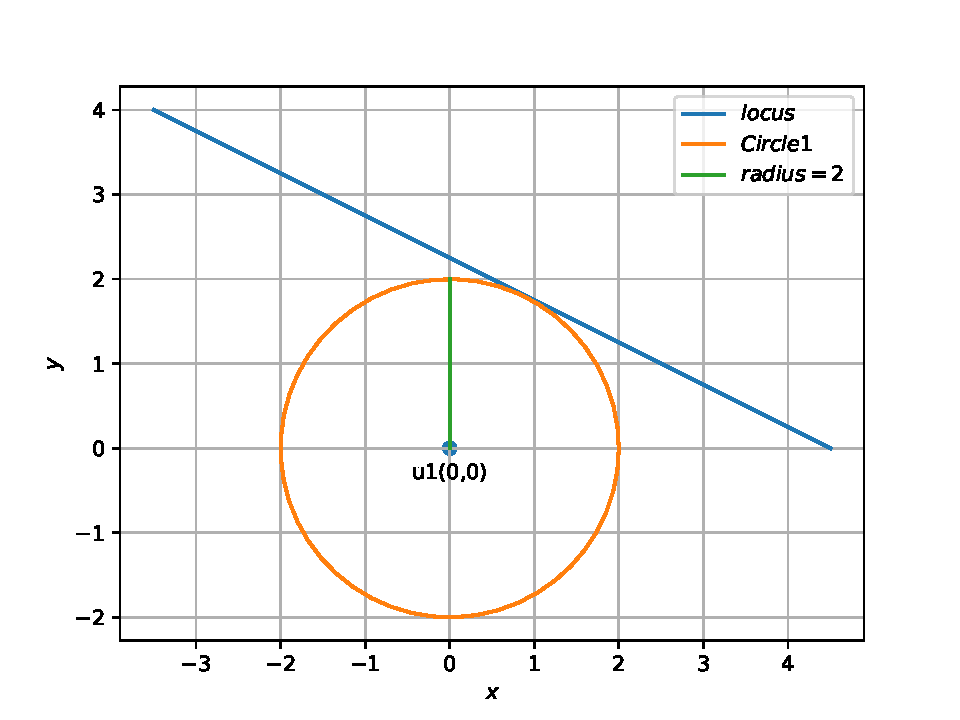
\includegraphics[scale=0.5]{/sdcard/Download/FWC-main/FWC-main/matrix/circle1.pdf} 


	\end{multicols}
\end{document}

